\documentclass[12pt]{article}
\usepackage[utf8]{inputenc}
\usepackage[T1]{fontenc}
\usepackage{titlesec}
\usepackage[inline]{enumitem}
\usepackage[left=2.54cm,top=3cm,right=2.54cm,bottom=3cm]{geometry}
\PassOptionsToPackage{hyphens}{url}\usepackage{hyperref}

\usepackage[sorting=none, style=numeric-comp]{biblatex}

\usepackage{pdfpages}
\usepackage{float}
\usepackage{graphicx}
\usepackage{tabularx}
\usepackage{setspace}
\usepackage{framed}
\usepackage{listings}
\usepackage{epigraph}
% \usepackage[table]{xcolor}
\usepackage[acronym,toc]{glossaries}

\renewcommand{\arraystretch}{1.15}


\graphicspath{ {00images/} }
\DeclareGraphicsExtensions{.png,.PNG,.pdf}
% \DeclareGraphicsExtensions{.pdf,.png,.PNG} % - CHANGE TO THIS

\addbibresource{references.bib}
\setlength{\parindent}{1cm}

% Acronyms %%%%%%%%
\makeglossaries

\newacronym{xacml}{XACML}{eXtensible Access Control Markup Language}
\newacronym{pdp}{PDP}{Policy Decision Point}
\newacronym{saml}{SAML}{Security Assertion Markup Language}
\newacronym{idp}{IdP}{Identity Provider}
\newacronym{rp}{RP}{Relying Party}
\newacronym{nist}{NIST}{National Institute of Standards and Technology}
\newacronym{pii}{PII}{Personally Identifiable Information}
\newacronym{ial}{IAL}{Identity Assurance Level}
\newacronym{csp}{CSP}{Credential Service Provider}
\newacronym{aal}{AAL}{Authenticator Assurance Level}
\newacronym{fal}{FAL}{Federation Assurance Level}
% \newacronym{}{}{}
% \newacronym{}{}{}
% \newacronym{}{}{}
% \newacronym{}{}{}
% \newacronym{}{}{}
% \newacronym{}{}{}
% \newacronym{}{}{}
% \newacronym{}{}{}

\makeglossaries

%%%%%%%%%%%%%%%%%%% 

\begin{document}

% \includepdf{cover_page}
% \includepdf{page_zero}
\tableofcontents

\begin{singlespacing}
\setglossarystyle{long}
\printglossary[type=\acronymtype, title=List of acronyms and abbreviations, toctitle=List of acronyms and abbreviations, nonumberlist]
\printglossary
\end{singlespacing}

% \section{Introduction}
% 
Access management systems (AMS) are playing a crucial role in every enterprise. They are being used/implemented for both, the physical access to company premises, online and internal resources. There are countless of different systems and providers offering such systems, ranging from simple card access systems and password log-ins to complex ones combining different types of physical and online access to resources. 

The problem of today’s access systems is that they are usually handling physical and online accesses separately, two systems have to be implemented and companies are usually specializing in providing one of those systems. Companies such as HID or G4S (check XYZ) are providing physical (AMS) to enterprises which allows employees to access the building, rooms, canteen or garage based on their access levels. On the other hand, there are tech companies such as Google or Microsoft which offer software for managing employees’ access to online services and resources.

Therefore, there exist two independent systems intended basically for the same use case. These systems are either managed individually or can be interconnected, so that there is one endpoint for managing accesses. Both approaches work fine, but what if there was an (AMS) which would combine both physical and online access? What if physical access would be possible by authenticating the employee with smartcard, smartphone or authenticator key? Simply, there would be a need only for one device, with which an employee would be able to access premises as well as authenticate himself when login-in. Such a system not only solves the problem of the employees’ experience and convenience of having to carry around an access card, but also a problem of security of enterprise account because of passwords. The reason is that many companies has policy that requires changes od password a few times a year and therefore employees tend to use easy to remember passwords  as well as many enterprise accounts has been “hacked” by phishing attacks . This can be avoided by using physical authenticators instead of passwords.

The aim of this project is to address this problem and propose a system, where physical access control and online access control will be managed from the single endpoint as it can be seen in Figure~\ref{fig:IntroArchitecture}. Another very important feature introduced by this system, is the possibility of using FIDO2 NFC enabled authenticator or smartphone to access a building, rooms or printers. Both devices would work similarly to an access card which is usually given to an employee. A device needs to be swiped in front of the reader which allows or deny access. It is common these days, that employees get to use many online services with their enterprise credentials/account. To avoid passwords, technology called FIDO2 aims to get rid of passwords when logging into account by using an authenticator, either a physical key device or smartphone. This allows “strong credentials” (check the term XYZ). The only thing the employee needs to type when logging-in is the username/e-mail and then he needs a FIDO2 authenticator which authenticates him, at least in our system. Because of that, the employee has no longer to carry an access card with him, and only needs smartphone or authenticator when accessing physical premises of enterprise, as well as it empowers him to “forget” about passwords when logging-in into online services by using the same smartphone and authenticator.

Secondary aim of this system lies in the access management, which allows or deny the entry or use of a service for an employee. To facilitate this, policies and role-based access will be implemented, which allows for assigning each employee a role/s and to create policies by which the access will be allowed or denied automatically.

\begin{figure}[ht]
    \centering
    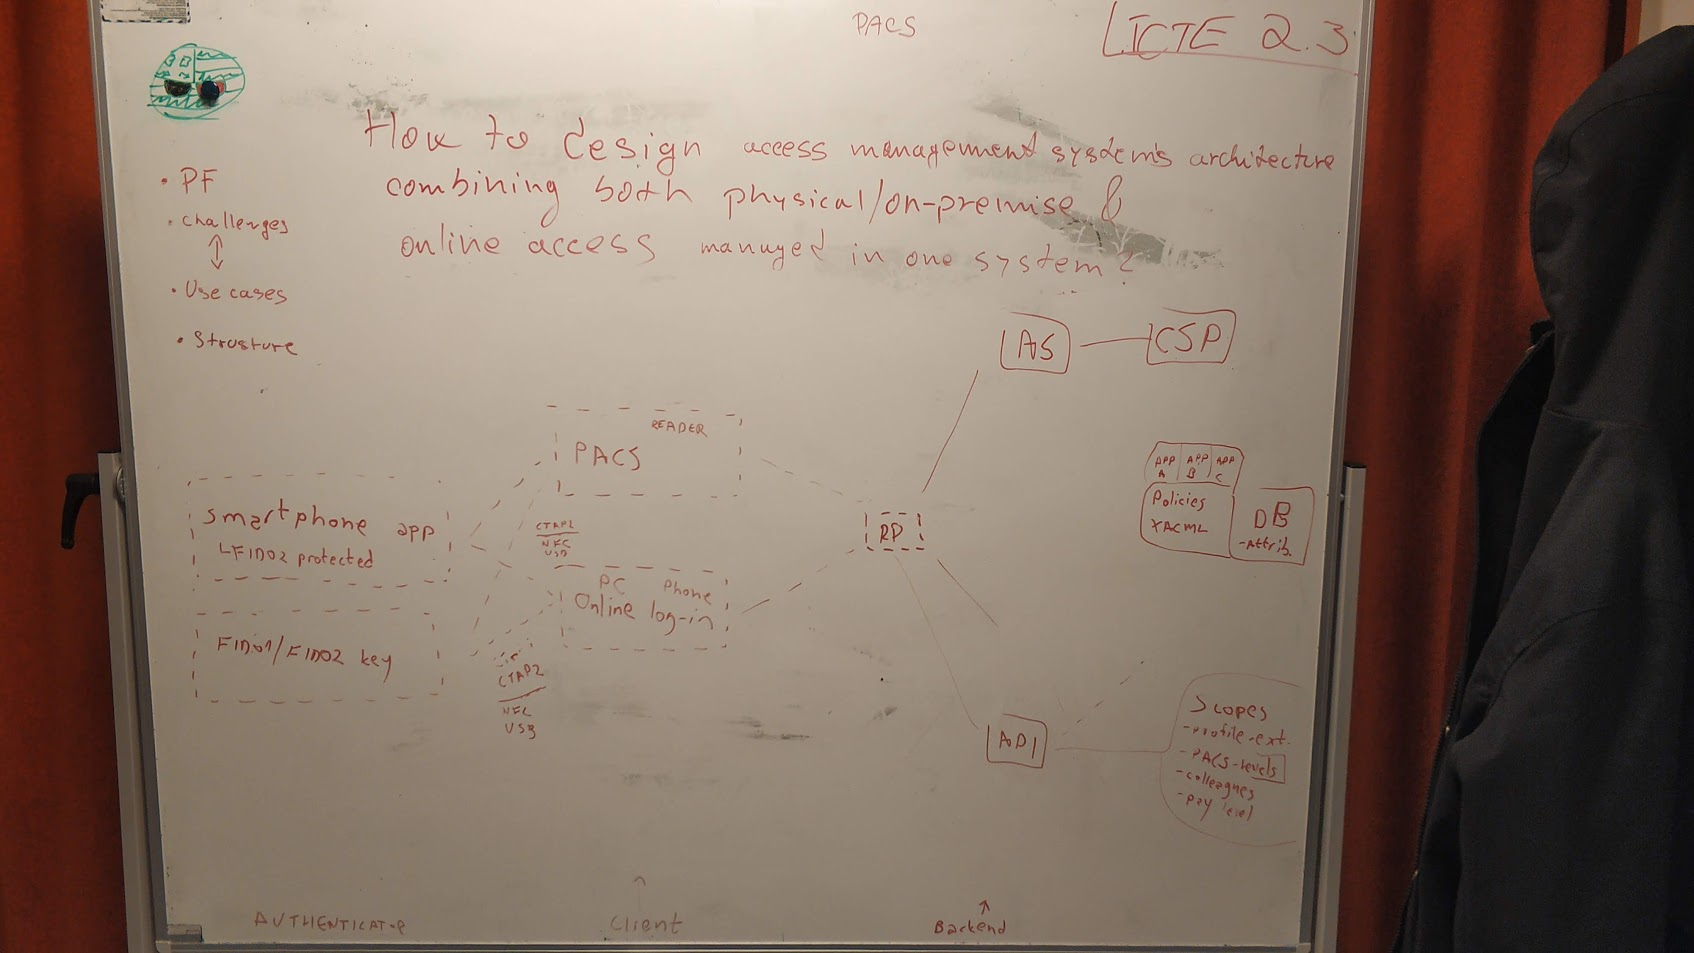
\includegraphics[width=.95\textwidth]{00images/IntroArchitecture}
    \caption{Explanation! + new diagram}
    \label{fig:IntroArchitecture}
\end{figure}

% \pagebreak
\section{Background}

% TODO section intro

\subsection{Basic terms}

\paragraph{Policy}
The IT portfolio of many current enterprises consists of a variety of different applications and systems. As a fine grained control of users' access to these resources is required, management of access rights for every user can become tedious. A set of rules is usually in place, which specify how a \textit{subject} (a person, user, actor) can interact with an \textit{object} (system, program), describing subject's accountability and capabilities within the object~\cite{Feltus2008PreliminaryConcept}. Policies are often used in the \hyperref[sec:xacml]{XACML} context.

\paragraph{Assertion}
An assertion is a ``confident and forceful statement of fact or belief''\footnotemark. In the context of authentication and in particular \hyperref[sec:saml]{SAML}, it is often the case that the identity provider is an independent entity, logically and physically separated from the application/relying party that requested user authentication. After the identity provider authenticates the user, it issues an assertion, confirming that the user's identity has been verified.

\footnotetext{\url{https://en.oxforddictionaries.com/definition/assertion}, accessed 05 March 2019}

\subsection{XACML}

 \acrfull{xacml} is a standardised, XML-based language for expressing security policies. It provides methods to define and combine security policies and to rapidly identify, which policy applies to a given subject. \acrshort{xacml} was first standardised by OASIS\footnote{\url{https://www.oasis-open.org/}, accessed 04 March 2019} in 2003 and the latest version is XACML 3.0, standardised in 2013~\cite{OASISStandard2013EXtensible3.0}. The further description is based on this latest version.
 
 The context of \acrshort{xacml} is illustrated in Figure~\ref{fig:xacml-context}. At the centre of the system is the \acrfull{pdp} which evaluates an input (such as access requests) against a policy set and issues an output -- a decision (such as \textit{access granted}). \acrshort{xacml} defines the formal language of the policy set and of the requests/responses. A policy set contains comprises one or more \textit{policies} and a \textit{policy combining algorithm}. The main components of a policy are a \textit{target} to which this policy applies and one or more \textit{rules}. The rule must specify a \textit{target} to which it applies and an \textit{evaluation} (\textit{permit} or \textit{deny}). It can also optionally specify \textit{conditions}, \textit{obligations} and \textit{advices}, all of which further shape the scope of the rule. Policy combining algorithm specifies the order and other conditions that decide, which policy will be finally applied on the request~\cite{OASISStandard2013EXtensible3.0}.
 
 \begin{figure}[ht]
    \centering
    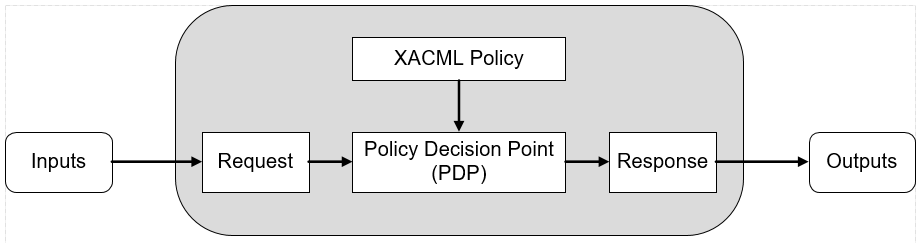
\includegraphics[width=.95\textwidth]{xacml-context}
    \caption{The context diagram of \acrshort{xacml}. From~\cite{OASISStandard2013EXtensible3.0}, edited.
    }
    \label{fig:xacml-context}
\end{figure}
 
The \acrshort{xacml} standard defines in detail several logical entities and their interactions. The native format for messages between these entities is XML, but a profile has been developed to support JSON message format~\cite{2017JSON1.0}. Additional profile was also created to describe implementation in a RESTful architecture~\cite{2017REST1.0}.
 
 Several implementations of \acrshort{xacml} exist in Java, Python and other languages. Criticisms of \acrshort{xacml} include low adoption rate, unsuitability for federated enterprises~\cite{Cser2013XACMLDead}, and lack of transparency for the end user~\cite{Cser2013XACMLDead, Ardagna2011ExpressiveApplications}.


\subsection{SAML}\label{sec:saml}

The \acrfull{saml} is a framework for exchange of assertions containing security information between two online parties, typically an identity provider and a relying party. Similarly as XACML, \acrshort{saml} was developed by OASIS. Version 1.0 was released in 2002 and version 2.0 (latest) in 2005. The rest of this report refers to version 2.0.

The main premise of \acrshort{saml} is that the \acrfull{idp} and the protected resource/application are two separated entities. This is desired, since it enables us to manage identities centrally for multiple applications and avoids duplication user accounts across these applications. Moreover, separating these enables both parts to specialise only in their task.

The Figure~\ref{fig:saml-architectire} illustrates the separation of these two entities. It also depicts the high-level flow of the authentication process. If the user wants to access the protected resource on the right, they first need to authenticate themselves with the \acrshort{idp}.

Another noteworthy aspect of \acrshort{saml} is the identity federation. This is achieved, when the \acrshort{idp} and the \acrshort{rp} are in different security realms, possibly operated by different organisations. As long as an agreement is established between the two, users can use identity managed by the \acrshort{idp} to access any resources outside the organisation's boundary~\cite{2008SecurityOverview}.

 \begin{figure}[ht]
    \centering
    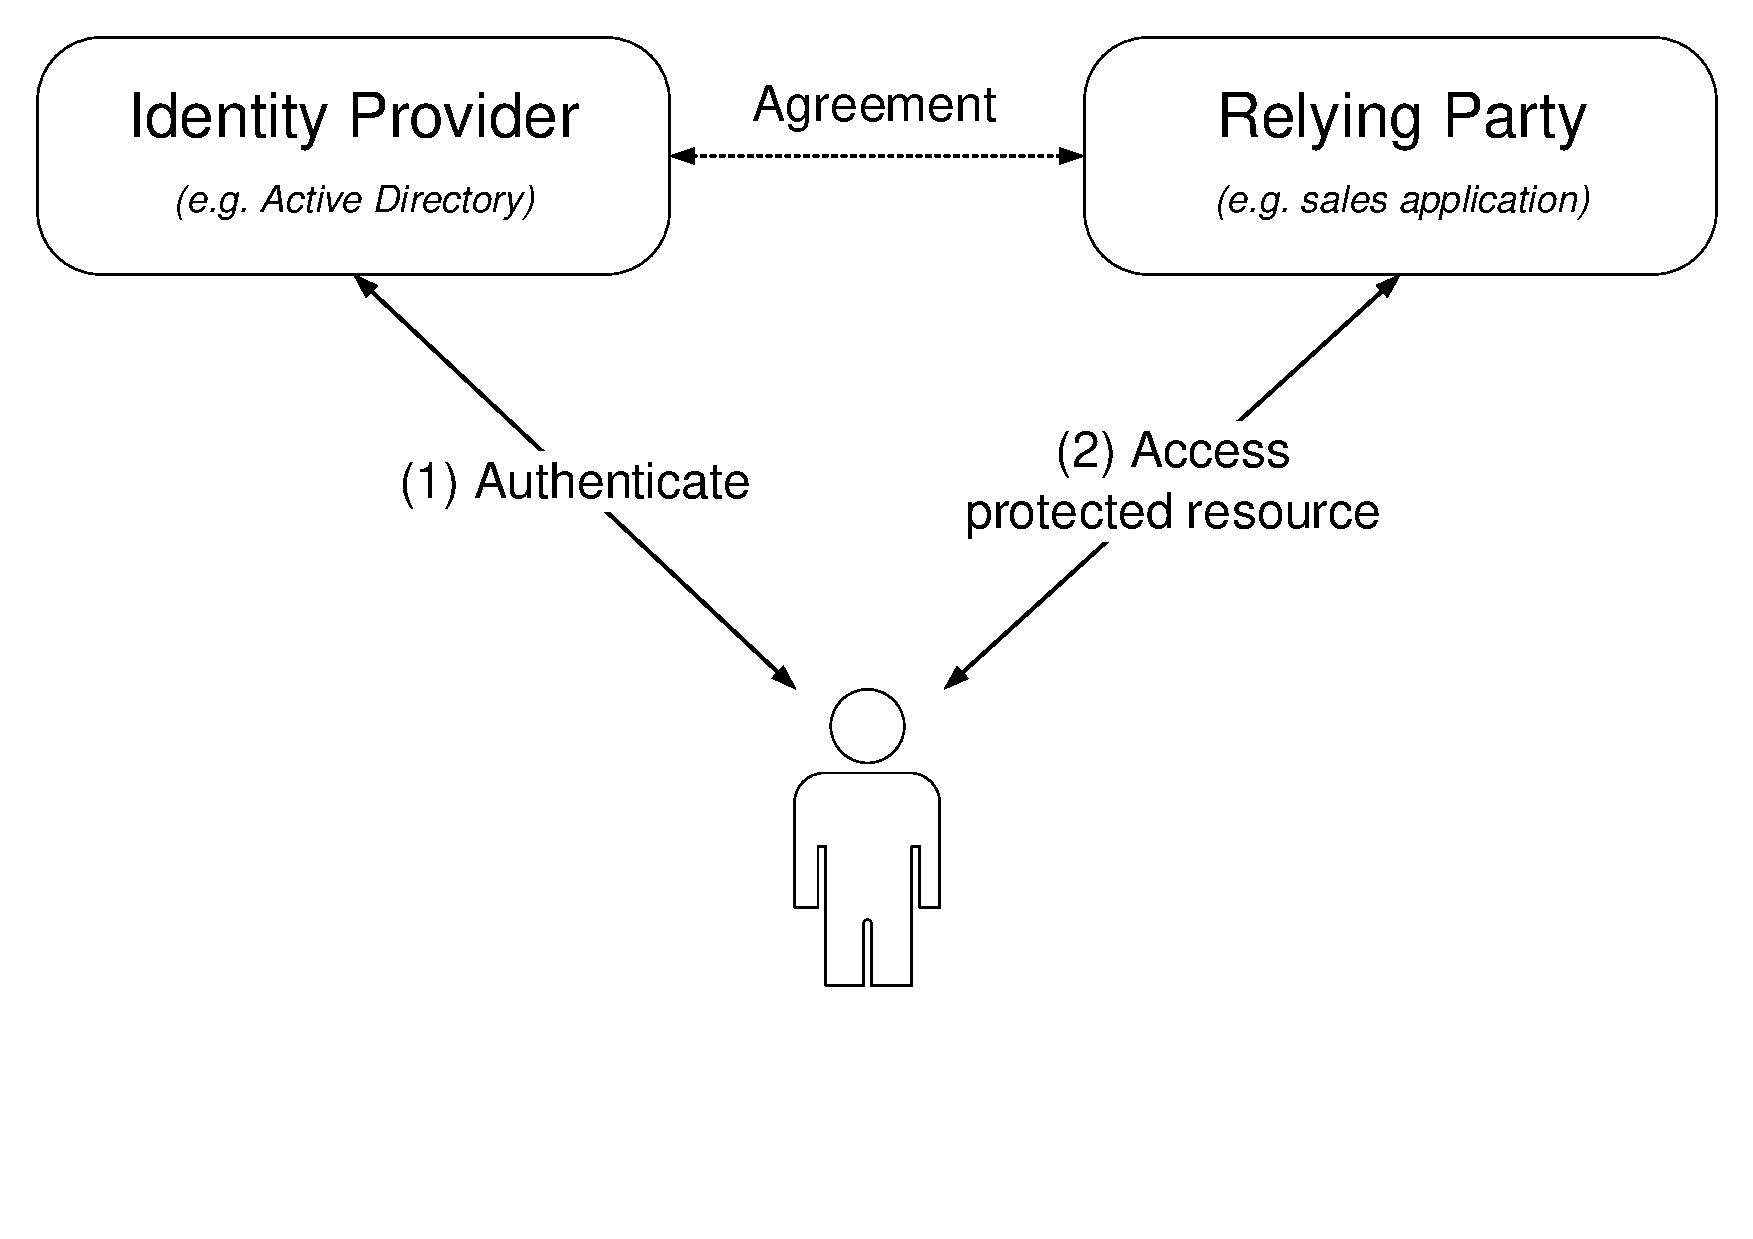
\includegraphics[width=.95\textwidth]{saml-architecture}
    \caption{The general use case of SAML, demonstrating the premise of functional separation of \acrshort{idp} and \acrshort{rp}. Taken from~\cite{2008SecurityOverview}.}
    \label{fig:saml-architectire}
\end{figure}

\paragraph{Assertions}
An assertion in \acrshort{saml} contains some security information about the \textit{subject}. Subject could be the user Bob and the associated information could be Bob's email address and job title. The security information need to be of one of following three categories:

\begin{enumerate*}[label=(\roman*)]
    \item \textit{Authentication statements} describe means and the timestamp of the authorisation carried out by the asserting party;
    \item \textit{Attribute statements} provide information about the subject; and
    \item \textit{Authorisation decision statement} describes what the subject is permitted to access in the system.
\end{enumerate*}

% \paragraph{Protocols}
% \acrshort{saml} defines a number of general protocols to facilitate the message exchange during different parts of the assertion process.

\paragraph{Bindings}
\acrshort{saml} describes how the messages exchanged during an assertion process can be bound to lower-level transport protocols. There are in total 6 bindings defined by the standard, but the following three are of particular interest:

\begin{itemize}[noitemsep]
    \item \textit{HTTP Redirect Binding}, where the entire \acrshort{saml} message is carried in the URL parameters, in the header of an HTTP GET method. This is suitable for short messages as the length of URL is limited in practice. This binding can be used in a RESTful system.
    \item \textit{HTTP POST Binding}, where the \acrshort{saml} message is base64 encoded into an XHTML form and transmitted using the HTTP POST method. This binding can also be used in a RESTful system.
    \item \textit{SAML SOAP Binding} specifies how the \acrshort{saml} messages are carried in an XML envelope over SOAP over any underlying transport protocol~\cite{Cantor2005BindingsV2.0}.
\end{itemize}

% \paragraph{Profiles}
% Several profiles which build on assertions and bindings are defined in the standard which correspond to the most common use cases of \acrshort{saml}. 

While \acrshort{saml} is widely adopted in the industry and is considered generally secure, numerous security flaws have been identified over time. Most of these arised from improper implementation of the protocol and have been patched since discovery~\cite{Krawczyk2014SecureAttacks}. The vulnerabilities included XML signature wrapping, assertion eavesdropping~\cite{Chen2014Environment-BoundAssertions} and XML parsing issues~\cite{Degges2018AVulnerability}.
\subsection{NIST Digital Identity Guidelines}

The \acrfull{nist} developed a set of guidelines, intended primarily to govern how public authorities in the US implement digital authentication in non-national-security scenarios. Yet, it was adopted by by wider community, spanning out of the government sector.
% REFERENCE Government Adopts an Industry Approach to Open Source Collaboration

The guidelines contain three volumes, covering three distinct areas of authentication:
\begin{enumerate*}[label=(\roman*)]
    \item SP 800-63A focused on Enrolment and Identity Proofing;
    \item SP 800-63B centred around Authentication and Lifecycle Management; and
    \item SP 800-63C covering federation and assertions.
\end{enumerate*}
The guidelines advertise the use of authentication to mitigate risks of unauthorised access to protected resources, but also promote minimising the collection of \acrfull{pii} and use of pseudonymous information whenever possible.
%REFERENCE Digital identity guidelines: revision 3

The guidelines define a Digital Identity Model (Figure~\ref{fig:nist-model}), which is useful to distinguish the various types of roles and activities within an authentication system. On the left side of the model there is a \acrfull{csp}. \acrshort{csp} is an entity that issues electronic credentials and registers user's \textit{authenticator} (authenticator is something that the user has or controls). On the right side of the model is the verifier, whose task is to authenticate users by validating binding of their authenticators to their credentials.
% %REFERENCE Digital identity guidelines: revision 3

 \begin{figure}[ht]
    \centering
    % TODO Change figure in visio
    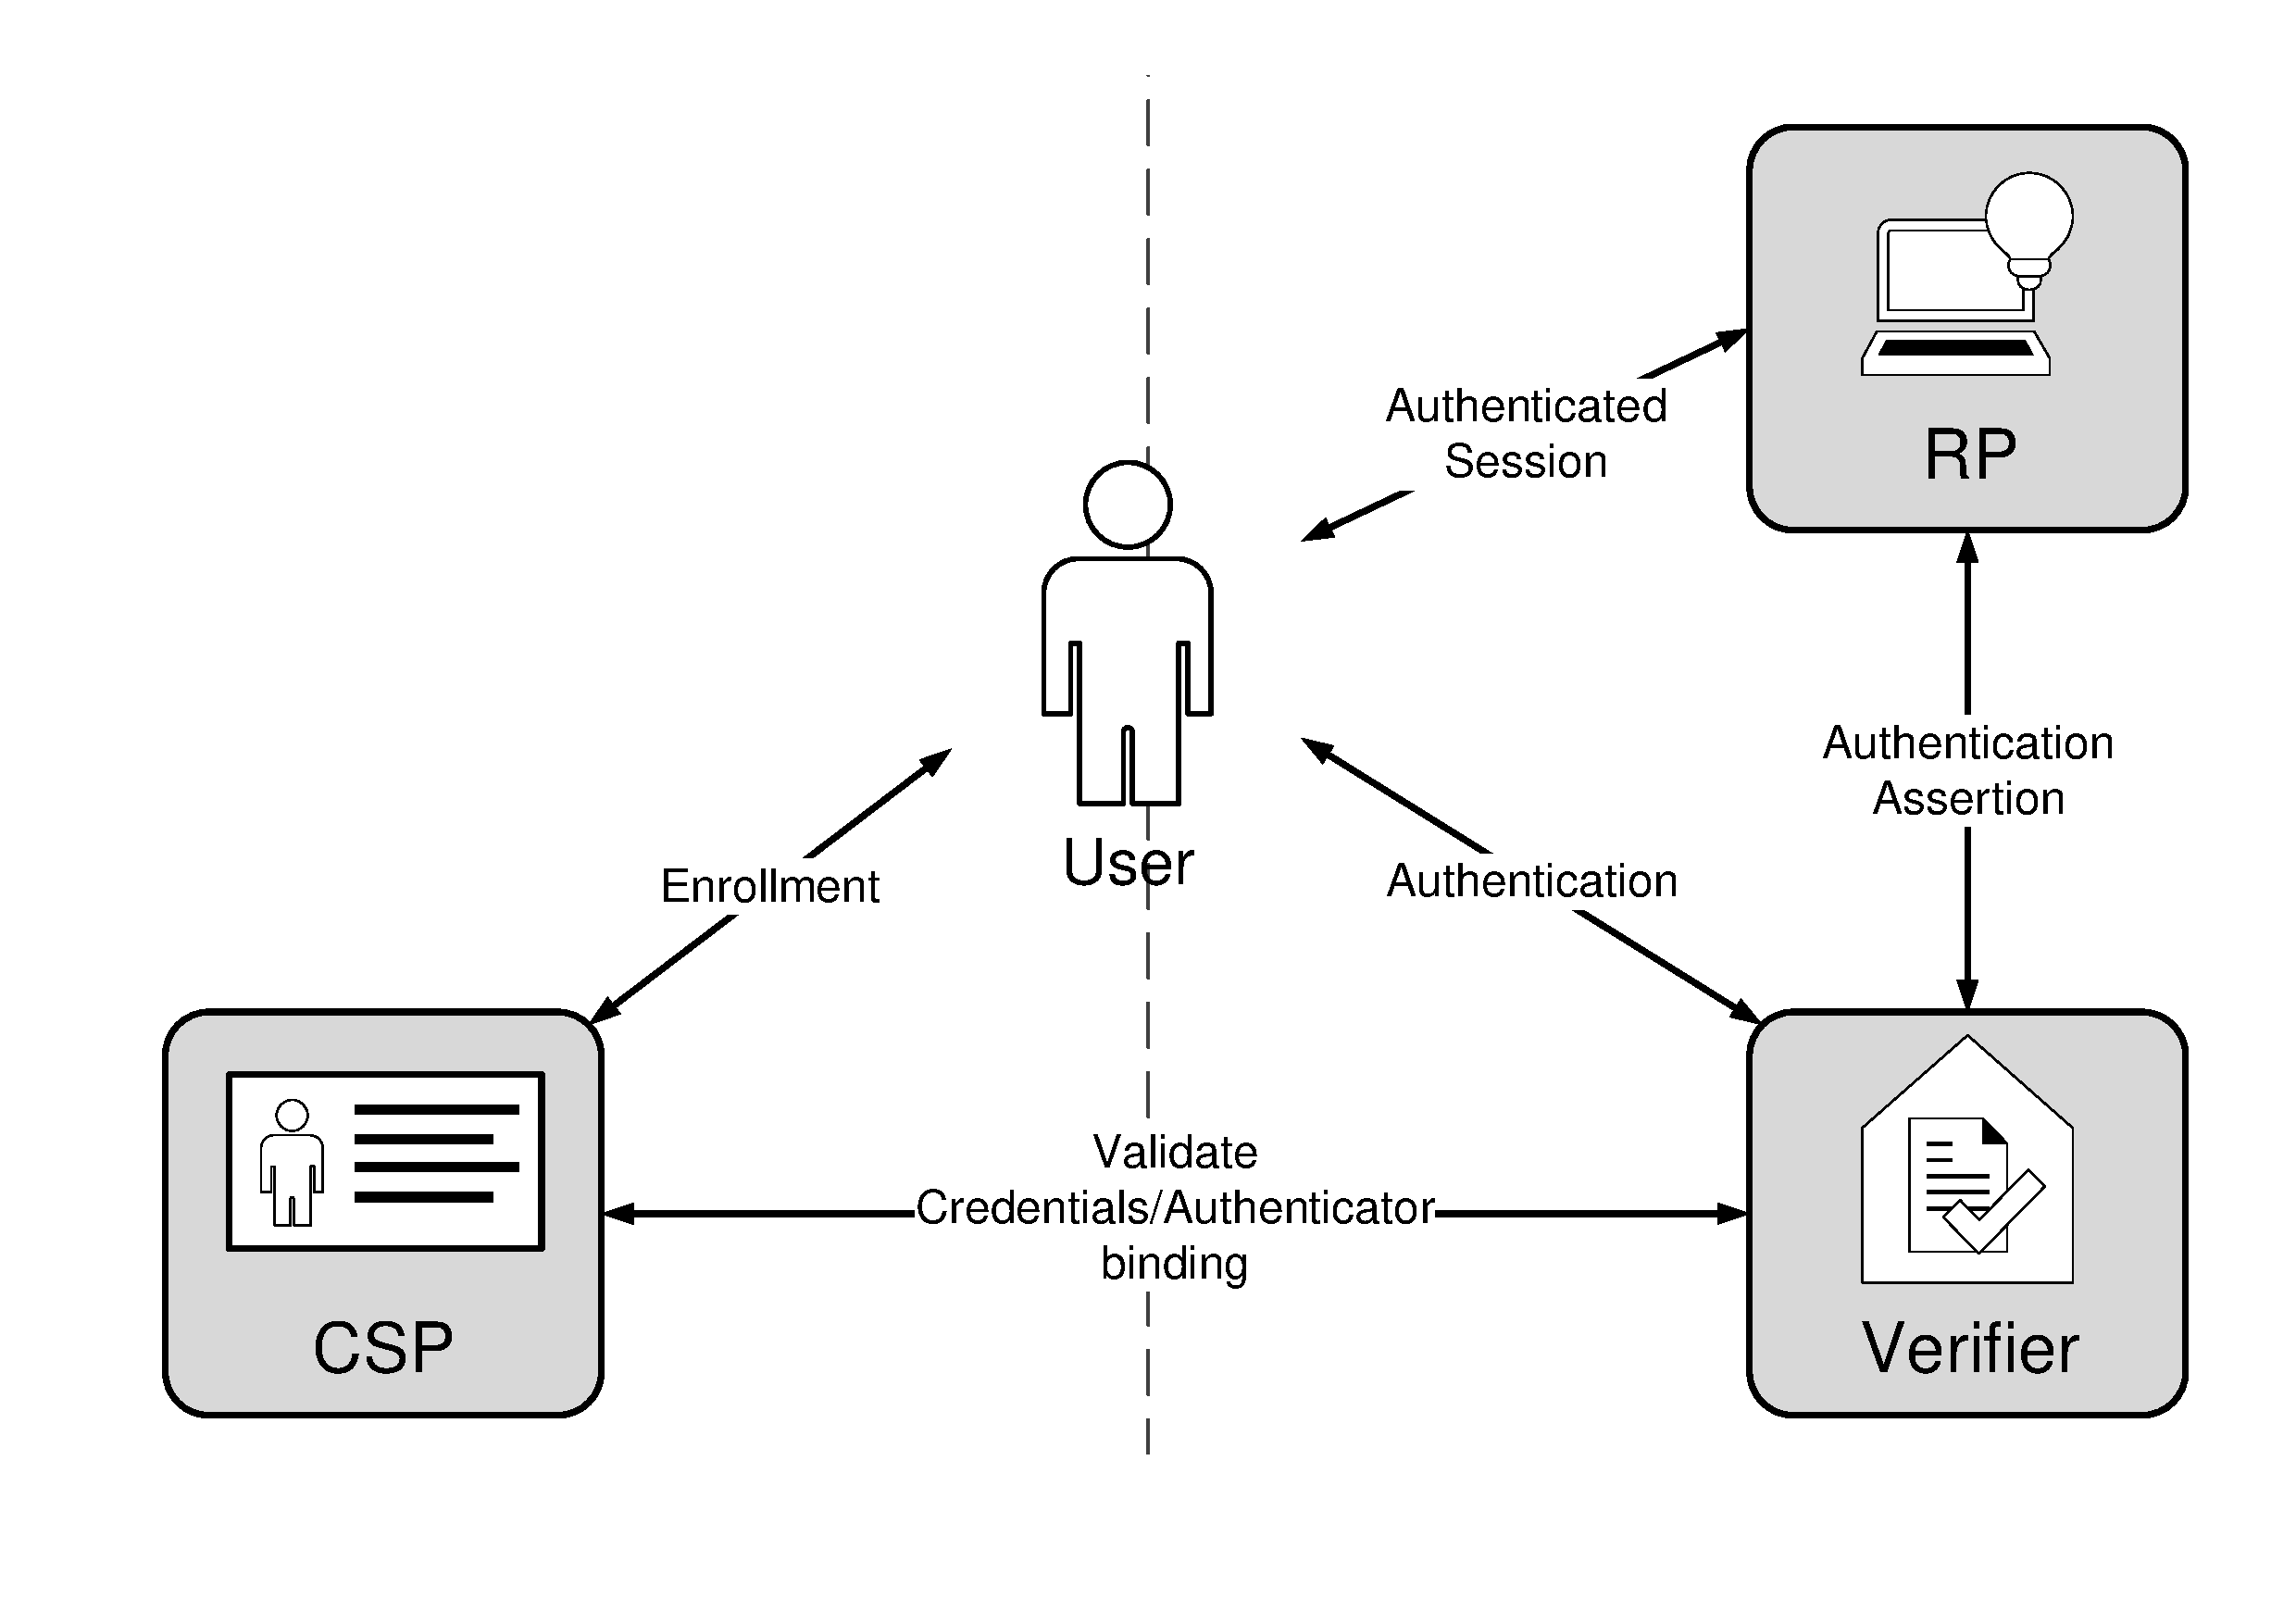
\includegraphics[width=.95\textwidth]{nist-simplified}
    \caption{Digital Identity Model (simplified). The left side of the figure represents enrolment of the user with the \acrshort{csp}. The right part of the user represents authentication with the verifier, before an authenticated session is established between the user and the \acrshort{rp}. Taken from (edited).
    % %REFERENCE Digital identity guidelines: revision 3
    }
    \label{fig:nist-model}
\end{figure}

\paragraph{SP 800-63A}
This volume of the Digital Identity Guidelines defines three Identity Assurance Levels (IALs) and requirements on identity proofing for each level. The \acrshort{ial}1 requires no verification of assertions provided by the user. \acrshort{ial}2 requires either remote or physically-present verification of assertions made by the user, while \acrshort{ial}3 requires manual verification by a trained person, representing the \acrshort{csp}.

% REFERENCE Digital identity guidelines: enrollment and identity proofing

\paragraph{SP 800-63B}
The B volume of the Guidelines defines three Authenticator Assurance Levels (AALs).

To authenticate themselves in AAL1, the user needs to demonstrate control of one authenticator. This must be done through a secure authentication protocol.

In AAL2, the user must demonstrate control of two distinct authenticators. This can be in a form of a multi-factor authenticator, or single-factor possession-based authenticator together with a memorised password. Cryptographic techniques defined in
% REFERENCE SECURITY REQUIREMENTS FOR CRYPTOGRAPHIC MODULES
must be used.

In AAL3, a hardware-based authenticator must be used in addition to requirements of AAL2. Furthermore, one of the authenticators used must be resistant to attacks attempting to impersonate the user.

\paragraph{SP 800-63C}
The C volume of the guidelines describes the use of assertions for identity federation across several \acrshort{rp}s. This enables the user to use services provided by several \acrshort{rp}s, while maintaining only a single identity at one \acrshort{idp}. The volume also describes three Federation Assurance Levels, however we do not cover these in this report.
% REFERENCE Digital identity guidelines: federation and assertions

\paragraph{Authenticator types}

% TODO WRITE HERE

\pagebreak
\section{Conclusion}\label{sec:conclusion}
Conclusion to be written
% TODO write conclusion

% A number of challenges arose when working on the project. The most fundamental challenge was to understand how \acrshort{acs} works, to identify its main components and to learn about the current systems. Once the knowledge is acquired, the selection of right technologies was an important aspect, as there exists many technologies and standards which can be implemented in the proposed system and therefore, finding the most suitable one was of a big importance. This goes hand in hand with designing a system’s architecture from the scratch and figuring out how the chosen components and technologies can be interconnected to perform desired tasks, while keeping in mind the security and easiness of use.
\pagebreak

\printbibliography[heading=bibintoc]

% \epigraph{Smart contracts are neither smart, nor contracts!}{\textit{www.stateofthedapps.com/about}}

\pagebreak

% \appendix
% \newgeometry{left=1cm,right=1cm,top=1cm,bottom=1cm,footskip=.4cm}
% \section{Operating System Market Share Worldwide}
\begin{figure}[H]
    \centering
    \includegraphics[height=0.6\textwidth, angle=90]{os-stats}
    \caption{Source: \url{http://gs.statcounter.com/os-market-share}, accessed 02-05-2018}
    \label{fig:os-stats}
\end{figure}
\restoregeometry
% \newgeometry{left=1cm,right=1cm,top=1cm,bottom=1cm,footskip=.4cm}
% \section{Smart contract code}\label{sec:appendix-code}
\begin{figure}[H]
    \centering
    \includegraphics[height=0.90\textheight]{code-smart-contract}
    \label{fig:smart-contract-code}
\end{figure}
\restoregeometry
% \newgeometry{left=2cm,right=2cm,top=1cm,bottom=1cm,footskip=.4cm}
% \section{Implemented requirements table}\label{sec:appendix-table}
\begin{table}[H]
    \centering
    \begin{tabularx}{\textwidth}{|l X c|}
    \hline
    \textbf{ID}&\textbf{Description}&\textbf{Implemented}\\
    % 
    \multicolumn{3}{|c|}{\textbf{Application front end}}\\
    AF-FR-1&Application must deploy the smart contract to an Ethereum node.&Yes\\
    AF-FR-2&Application must be able to query the node for address balance.&Yes\\
    AF-FR-3&Application must display the status of the transaction.&Yes\\
    AF-NFR-1&Transaction must be signed on device.&Yes\\
    AF-NFR-2&Sensitive details about users' funds must not leave the device.&Yes\\
    % 
    \multicolumn{3}{|c|}{\textbf{Ethereum node}}\\
    EN-FR-1&Node must support at least the following methods of the JSON-RPC protocol: \texttt{eth\_getBalance} and \texttt{eth\_sendTransaction}.&Yes\\
    EN-NFR-1&Node should process method calls without delay.&\textbf{No}\\
    EN-NFR-2&Node should process all method calls with equal priority.&\textbf{No}\\
    EN-NFR-3&Node should inform the application about the outcome of the method call.&\textbf{No}\\
    % 
    \multicolumn{3}{|c|}{\textbf{Smart contract}}\\
    SC-FR-1&The smart contract must implement the logic described in~\ref{fig:simple-logic}.&Yes\\
    SC-NFR-1&The smart contract must emit en event after contract creation.&Yes\\
    SC-NFR-2&The smart contract must cover the costs for the services of the oracle.&\textbf{No}\\
    SC-NFR-3&The smart contract could emit an event upon receiving a response from the oracle.&Yes\\
    % 
    \multicolumn{3}{|c|}{\textbf{Oracle}}\\
    OR-FR-1&The oracle must support queries to a web \acrshort{api}.&Yes\\
    OR-NFR-1&The oracle should provide accurate and correct response to the query.&\textbf{No}\\
    OR-NFR-2&The oracle should respond to queries without delay (unless otherwise specified).&\textbf{No}\\
    %   
    \multicolumn{3}{|c|}{\textbf{Blockchain explorer}}\\
    BE-FR-1&Blockchain explorer must support an API query for address balance.&Yes\\
    BE-NFR-1&The blockchain explorer should provide accurate and correct response to the query.&\textbf{No}\\
    BE-NFR-2&The blockchain explorer should respond to queries without delay.&\textbf{No}\\
    % 
    \multicolumn{3}{|c|}{\textbf{Communication back end}}\\
    CB-FR-1&Communication back end should be able to store users' offers.&Yes\\
    CB-FR-1&Communication back end should assist users during the transaction process.&Yes\\
    CB-NFR-1&The communication back end must not be able to prevent a transaction from happening.&\textbf{No}\\
    CB-NFR-2&The communication back end must not have control over users' funds.&Yes\\
    \hline
    \end{tabularx}
    % \caption{//write}
    \label{tab:component-reqs-eval}
\end{table}

% \newgeometry{left=1cm,right=1cm,top=1cm,bottom=1cm,footskip=.4cm}
% \section{Transaction process screenshots}\label{sec:appendix-screenshots}

% //ADD Screensoht descriptions

    \centerline{\includegraphics[width=0.75\textwidth]{screenshots/screen020}}
    \centerline{\includegraphics[width=0.75\textwidth]{screenshots/screen031}}
    \textit{Top:}    Front page of the application\\
    \textit{Bottom:} The secondary user clicked on \textit{Create new offer}.\\
    \centerline{\includegraphics[width=0.85\textwidth]{screenshots/screen032}}
    \centerline{\includegraphics[width=0.85\textwidth]{screenshots/screen033}}
    \textit{Top:}    The secondary user filled in the details of the Bitcoin offer.\\
    \textit{Bottom:} The secondary user clicked on \textit{OR} button to scan the destination Ethereum address.\\
    \centerline{\includegraphics[width=0.85\textwidth]{screenshots/screen034}}
    \centerline{\includegraphics[width=0.85\textwidth]{screenshots/screen041}}
    \textit{Top:}    The Ethereum address was filled by the QR code scan.\\
    \textit{Bottom:} The secondary user clicked on \textit{Create new offer}.\\
    \centerline{\includegraphics[width=0.85\textwidth]{screenshots/screen042}}
    \centerline{\includegraphics[width=0.85\textwidth]{screenshots/screen043}}
    \textit{Top:}    The primary user selected the offer from the list.\\
    \textit{Bottom:} The primary user clicked on \textit{Continue}. A screen prompting them to transfer funds to said Ethereum address was displayed.\\
    \centerline{\includegraphics[width=0.85\textwidth]{screenshots/screen051}}
    The primary user clicked on \textit{Continue}. A screen prompting them to fill in their Bitcoin address was displayed. The Ethereum address and Bitcoin address are pre-filled.\\
    \centerline{\includegraphics[width=0.85\textwidth]{screenshots/screen060}}
    The primary user deposited Ether to the temporary Ethereum address.\\
    \centerline{\includegraphics[width=0.85\textwidth]{screenshots/screen071}}
    \centerline{\includegraphics[width=0.85\textwidth]{screenshots/screen072}}
    \textit{Top:}    The balance of the temporary Ether wallet has changed.\\
    \textit{Bottom:} The primary user filled in their Bitcoin address.\\
    \centerline{\includegraphics[width=0.80\textwidth]{screenshots/screen081}}
    \centerline{\includegraphics[width=0.80\textwidth]{screenshots/screen082}}
    \textit{Top:}    The primary user clicked on \textit{Validate}. This displayed a validation screen and triggered a prompt at the secondary user's device.\\
    \textit{Bottom:} Secondary user pressed \textit{Yes}. This action changed the colour of the \textit{Yes} button on primary user's screen.\\
    \centerline{\includegraphics[width=0.80\textwidth]{screenshots/screen091}}
    \centerline{\includegraphics[width=0.80\textwidth]{screenshots/screen092}}
    \textit{Top:}    A transaction hash was displayed to the primary user and a link to blockchain explorer was displayed to both users.\\
    \textit{Bottom:} The secondary user clicked on \textit{Continue}. This displayed a screen, prompting them to transfer the Bitcoin\\    
    \centerline{\includegraphics[width=0.85\textwidth]{screenshots/screen100}}
    The secondary user transferred the Bitcoin to the primary user.\\
    \centerline{\includegraphics[width=0.85\textwidth]{screenshots/screen110}}
    Response from Oraclize.
    

% \restoregeometry

\end{document}